\documentclass[tikz,border=3mm,multi=tikzpicture]{standalone}
\usepackage[utf8]{inputenc}
\usepackage[T1]{fontenc}
\usepackage{helvet}
\renewcommand{\familydefault}{\sfdefault}
\usepackage{tikz}
\usetikzlibrary{arrows.meta,positioning}
\begin{document}

\tikzset{every node/.append style={font=\sffamily\small}}

% TikZ 1
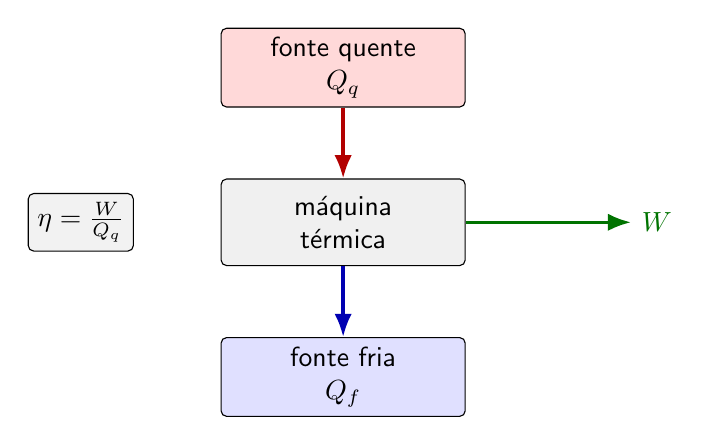
\begin{tikzpicture}[>=Latex,node distance=0.9cm]
  \node[draw,rounded corners=2pt,fill=red!15,minimum width=3.1cm,minimum height=0.9cm,align=center] (quente)
    {fonte quente\\$Q_q$};
  \node[draw,rounded corners=2pt,fill=gray!12,minimum width=3.1cm,minimum height=1.1cm,align=center,below=of quente] (maq)
    {máquina\\térmica};
  \node[draw,rounded corners=2pt,fill=blue!12,minimum width=3.1cm,minimum height=0.9cm,align=center,below=of maq] (fria)
    {fonte fria\\$Q_f$};
  \draw[very thick,->,red!70!black] (quente) -- (maq);
  \draw[very thick,->,blue!70!black] (maq) -- (fria);
  \draw[very thick,->,green!45!black] (maq.east) -- ++(2.1,0) node[right] {$W$};
  \node[draw,rounded corners=2pt,fill=gray!10,align=center,left=1.1cm of maq]
    {$\eta=\frac{W}{Q_q}$};
\end{tikzpicture}

% TikZ 2
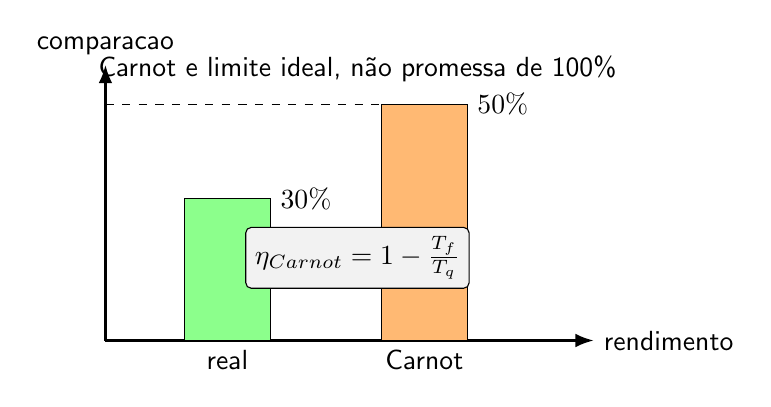
\begin{tikzpicture}[x=1cm,y=1cm,>=Latex]
  \draw[->,thick] (0,0) -- (6.2,0) node[right] {rendimento};
  \draw[->,thick] (0,0) -- (0,3.5) node[above] {comparacao};
  \draw[fill=green!45] (1,0) rectangle (2.1,1.8);
  \draw[fill=orange!55] (3.5,0) rectangle (4.6,3.0);
  \node[below] at (1.55,0) {real};
  \node[below] at (4.05,0) {Carnot};
  \node[right] at (2.1,1.8) {$30\%$};
  \node[right] at (4.6,3.0) {$50\%$};
  \draw[dashed] (0,3) -- (4.6,3);
  \node[align=center] at (3.2,3.45) {Carnot e limite ideal, não promessa de 100\%};
  \node[draw,rounded corners=2pt,fill=gray!10,align=center] at (3.2,1.05)
    {$\eta_{Carnot}=1-\frac{T_f}{T_q}$};
\end{tikzpicture}

\end{document}
